\documentclass[10pt,times,twocolumn]{article}

\usepackage{sbcm2019}
\usepackage{graphicx,url}
\usepackage{hyperref}
\usepackage{tikz}
\usetikzlibrary{arrows.meta}
\usepackage{biblatex}
\addbibresource{example.bib}
\usepackage[table]{xcolor}
\usepackage{float}
\usepackage[utf8]{inputenc}
\usepackage[spanish]{babel}
%\usepackage{booktabs} % Para líneas de tabla más profesionales
% -------------------------------------------------------
% Packages that facilitate double-blind peer review
% Comment the first line and uncomment the second to remove double-blindness
%\usepackage[blind]{anonymize} % Blind
\usepackage{anonymize} % not blind
% --------------------------------------------------------

\usepackage[spanish]{babel} 
\usepackage{fancyhdr} % Custom headers and footers
\pagestyle{fancyplain} % Makes all pages in the document conform to the custom headers and footers
\fancyhead{} 
\fancyfoot[C]{\thepage} % Page numbering for right footer
\usepackage{lipsum}
\setlength\parindent{0pt} 
\usepackage{amsmath,amsfonts,amsthm} % Math packages
\usepackage{wrapfig}
\usepackage{graphicx}
\usepackage{float}
\usepackage{subcaption}
\usepackage{comment}
\usepackage{enumitem}
\usepackage{cuted}
\usepackage{sectsty} % Allows customizing section commands
\allsectionsfont{\normalfont \normalsize \scshape} % Section names in small caps and normal fonts
\usepackage{hyperref}
\usepackage{xcolor}
\usepackage{siunitx}
\usepackage{icomma}
\usepackage{tikz}
\usetikzlibrary{arrows.meta}
\usepackage{listings}

\sloppy

\title{Desarrollo de un Tokenizador Mínimo para la Analítica de Voz en Interacciones Telefónicas en Español}

\author
{
	\anonymize{Elías Cristaldo}\inst{1} 	
}

\address{
	\anonymize{Ingeniería en Informática / 
	Facultad Politécnica / 
	Universidad Nacional de Asunción}\\
    \anonymize{Campus, San Lorenzo – Paraguay, Teléfono (+595-21) 588 7000}\\ \\
	\anonymize{\textit{27 de Junio del 2024\vspace{10pt}}}
}

\begin{document}

\maketitle

\begin{abstract}
Este informe propone una solución para la implementación de los analizadores de voz. Utilizando conocimientos fundamentales del análisis léxico, se construye un tokenizador mínimo que funciona como una herramienta de analítica de voz. Este tokenizador se encargará de identificar los lexemas presentes en un texto que representa la interacción de una llamada telefónica y asignará las etiquetas correspondientes. La solución se desarrolla en tres etapas principales: la primera etapa corresponde al análisis del personal de atención. En esta fase, el texto correspondiente al personal de atención es analizado, y como resultado, se obtiene una puntuación relativa al personal. Como segunda etapa tenemos el análisis del cliente, de vuelta se analiza el texto ingresado, pero en este caso realtiva al cliente, obteniendo así una puntuación que refleja el nivel relativo de satisfacción del cliente respecto a la solución de sus necesidades. Como tercera y última etapa tenemos el análisis global de la llamada, en esta etapa se realiza un análisis combinando las puntuaciones obtenidas en las etapas anteriores, ofreciendo una evaluación integral de la llamada. El programa propuesto demuestra un buen desempeño en el análisis léxico del texto recibido como entrada. Además, puede ser ampliado para mejorar su capacidad de detección de patrones y, al ser combinado con otros algoritmos, alcanzar niveles óptimos de rendimiento.\\

{\bf Keywords:} tokenizador mínimo, analítica de voz, análisis léxico, interacción telefónica, satisfacción del cliente, desempeño del personal, token.\\
\rule{\linewidth}{0.5pt}

\end{abstract}

% ------------------------------- INTRODUCCION -------------------------------
\section{Introducción}
En el ámbito de la analítica de conversaciones, la capacidad de procesar y analizar grandes volúmenes de interacciones telefónicas se ha vuelto una necesidad crítica para muchas organizaciones. Estas interacciones contienen una gran cantidad de información valiosa que puede ser utilizada para mejorar la calidad del servicio, entender mejor las necesidades de los clientes y optimizar procesos internos. 

Para abordar esta necesidad, presentamos el desarrollo de un tokenizador mínimo, conocido como MNLPTK (Minimal Natural Language Processing Tokenizer). Este sistema está diseñado para actuar como una solución de analítica de voz (speech analytics), con el objetivo de identificar y procesar palabras (lexemas) en textos en idioma español que son el resultado de conversaciones telefónicas.

El \textbf{MNLPTK} se enfoca en la identificación precisa de lexemas en los textos de entrada, lo cual es un paso fundamental en el procesamiento del lenguaje natural (NLP). Una vez identificados los lexemas, el sistema los procesará para generar una ponderación sobre la llamada en general. 
Esta evaluación se basará en varios criterios que, en cierta medida, reflejan la calidad y el contenido de la interacción.

\section{Objetivo, alcance y mejoras}


El objetivo de este proyecto es implementar un sistema de \textbf{Speech Analytics} que aproveche los conocimientos adquiridos en el análisis léxico de un compilador. Este sistema se diseñará para procesar y analizar datos de audio convertidos a texto, extrayendo información valiosa para la organización.

Aplicando principios de análisis léxico, se busca desarrollar un programa capaz de identificar patrones en las conversaciones y asignar puntuaciones coherentes a las llamadas. Este enfoque permitirá obtener un análisis detallado de la calidad del servicio y la atención al cliente, proporcionando información que pueda ayudar a mejorar continuamente el servicio ofrecido.

En cuanto al alcance del proyecto, se espera que el análisis se realice únicamente a nivel léxico. No se considerarán aspectos sintácticos ni semánticos, ya que el objetivo es desarrollar un tokenizador mínimo.

El programa podría potenciar su capacidad de aprendizaje mediante la implementación de enfoques más avanzados. Actualmente, no está diseñado para reconocer variantes de género y número en las palabras de entrada. Sin embargo, esta funcionalidad podría integrarse en futuras actualizaciones para mejorar la precisión y utilidad del análisis léxico. Además, es posible mejorar la ponderación de las palabras; actualmente, todas reciben el mismo peso, siendo asignadas como 1, -1 o 0 según su tipo.

% ------------------------------- METODOLOGIA -------------------------------
\section{Metodología}
Para la aplicación del \textbf{MNLPTK} se establecieron los siguientes puntos.

\subsection{Tokens definidos para el lenguaje de entrada}
El MNLPTK contará con los siguientes tokens: \textbf{EXP\_MALA}, \textbf{EXP\_NEUTRA}, \textbf{EXP\_BUENA} que irán destinados para el análisis de la interacción del cliente y \textbf{ATC\_MALA}, \textbf{ATC\_NEUTRA}, \textbf{ATC\_BUENA} que corresponderán a la interacción del personal de atención al cliente.

\subsection{Definición de la herramienta a utilizar para la definición de los patrones}
Para la representación de los patrones se opta por utilizar el algoritmo de simulación de un \textbf{AFD} \cite{compi2008} para obtener los lexemas. En la Figura \ref{fig:tokens} podemos observar una categorizacion de los tokens por colores de acuerdo si es una palabra buena, nuetral o mala. Esto último para entender a través de un ejemplo, el funcionamiento del algoritmo propuesto. 

\newcounter{i}
\setcounter{i}{0}

\definecolor{mala}{HTML}{FFBABA}
\definecolor{neutra}{HTML}{E0E0E0}
\definecolor{buena}{HTML}{DFF2BF}

\begin{figure}[H]
  \centering
  	\begin{tikzpicture}
    		\node[circle, draw, double, fill=mala, minimum height=1.8cm, 
        text width=1.8cm, align=center, inner sep=0] (mala) at (0,0) {MALA};
    		
    		\node[circle, draw, double, fill=neutra, minimum height=1.8cm, 
        text width=1.8cm, align=center, inner sep=0] (mala) at (2,0) {NEUTRA};
    		
    		\node[circle, draw, double, fill=buena,  minimum height=1.8cm, 
        text width=1.8cm, align=center, inner sep=0] (mala) at (4,0) {BUENA};
        
	\end	{tikzpicture}
	\caption{Tokens.}
	\label{fig:tokens}
\end{figure}

A continuación, en la Figura \ref{fig:afd} se muestra a través de un ejemplo, la estructura que se utilizará en la implementación del AFD. En esta representación, cada nodo que corresponda a un estado final estará asociado una categoría específica. Es importante destacar que habrán dos estructuras similares: una para la atención al cliente, que manejará los tokens ATC\_MALA, ATC\_NEUTRA y ATC\_BUENA. Otra otra para la experiencia del cliente, que incluirá los tokens EXP\_MALA, EXP\_NEUTRA y EXP\_BUENA.

\begin{figure}[H]
  \centering
  \begin{tikzpicture}
  
    % Nodos
    \node[circle, draw] (\arabic{i}) at (0,6) {\arabic{i}};
    \stepcounter{i}
	\node[circle, draw, double, fill=neutra] (\arabic{i}) at (1,6) {\arabic{i}};
    \stepcounter{i}
    	\node[circle, draw] (\arabic{i}) at (2,6) {\arabic{i}};
    \stepcounter{i}
    \node[circle, draw] (\arabic{i}) at (3,6) {\arabic{i}};
    \stepcounter{i}
    	\node[circle, draw] (\arabic{i}) at (4,6) {\arabic{i}};
    \stepcounter{i}
    \node[circle, draw, double, fill=buena] (\arabic{i}) at (5,6) {\arabic{i}};
    \stepcounter{i}
   	\node[circle, draw, double, fill=buena] (\arabic{i}) at (6,6) {\arabic{i}};
    \stepcounter{i}
    \node[circle, draw, double, fill=buena] (\arabic{i}) at (5,5) {\arabic{i}};
    \stepcounter{i}
    
   	\node[circle, draw] (\arabic{i}) at (1,4) {\arabic{i}};
    \stepcounter{i}
    \node[circle, draw] (\arabic{i}) at (2,4) {\arabic{i}};
    \stepcounter{i}
   	\node[circle, draw] (\arabic{i}) at (3,4) {\arabic{i}};
    \stepcounter{i}
   	\node[circle, draw] (\arabic{i}) at (4,4) {\arabic{i}};
    \stepcounter{i}
   	\node[circle, draw] (\arabic{i}) at (5,4) {\arabic{i}};
    \stepcounter{i}
   	\node[circle, draw, double, fill=mala] (\arabic{i}) at (6,4) {\arabic{i}};
    \stepcounter{i}
    
    \node[circle, draw] (\arabic{i}) at (2,3) {\arabic{i}};
    \stepcounter{i}
    \node[circle, draw] (\arabic{i}) at (3,3) {\arabic{i}};
    \stepcounter{i}
    \node[circle, draw] (\arabic{i}) at (4,3) {\arabic{i}};
    \stepcounter{i}
    \node[circle, draw, double, fill=buena] (\arabic{i}) at (5,3) {\arabic{i}};
    \stepcounter{i}
 
    \node[circle, draw] (puntos) at (1,2) {...};
    \node[circle, draw] (n) at (1,0) {n};
    
    % Aristas con flechas
    \draw[-{Stealth}] (0) -- node[midway, above] {a} (1);
    \draw[-{Stealth}] (1) -- node[midway, above] {y} (2);
    \draw[-{Stealth}] (2) -- node[midway, above] {u} (3);
    \draw[-{Stealth}] (3) -- node[midway, above] {d} (4);
    \draw[-{Stealth}] (4) -- node[midway, above] {a} (5);
    \draw[-{Stealth}] (5) -- node[midway, above] {r} (6);
    \draw[-{Stealth}] (4) |- node[near end, above] {o} (7);
    
    \draw[-{Stealth}] (0) |- node[near end, above] {b} (8);
    \draw[-{Stealth}] (8) -- node[midway, sloped, above] {a} (9);
    \draw[-{Stealth}] (9) -- node[midway, sloped, above] {s} (10);
    \draw[-{Stealth}] (10) -- node[midway, sloped, above] {u} (11);
    \draw[-{Stealth}] (11) -- node[midway, sloped, above] {r} (12);
    \draw[-{Stealth}] (12) -- node[midway, sloped, above] {a} (13);
    
    \draw[-{Stealth}] (8) |- node[near end, sloped, above] {u} (14);
    \draw[-{Stealth}] (14) -- node[midway, sloped, above] {e} (15);
    \draw[-{Stealth}] (15) -- node[midway, sloped, above] {n} (16);
    \draw[-{Stealth}] (16) -- node[midway, sloped, above] {o} (17);
    
    \draw[-{Stealth}] (0) |- node[near end, sloped, above] {...} (puntos);
    \draw[-{Stealth}] (0) |- node[near end, sloped, above] {ü} (n);
    
  \end{tikzpicture}
  \caption{Grafo dirigido con tres nodos.}
  \label{fig:afd}
\end{figure}

La idea es que todas las letras del abecedario tengan un único estado inicial. Esto permitirá que al recorrer la estructura, solo se necesite una función, la función \textbf{mover}. Esta función tomará un carácter de entrada y, en función del nodo en el que se encuentre, se moverá a un nuevo nodo.

\subsection{Estructura de los Nodos del AFD}
Para la construcción del AFD, se definió la estructura Nodo junto con sus atributos correspondientes. En la Figura \ref{fig:estructura_nodo} podremos apreciar con más detalles la mencionada estructura.

\begin{figure}[H]
	\begin{tikzpicture}
	
		% Nodos
		\node (atributos) at (3, 5) {Atributos};
		\node (estructuras) at (7,5) {Estructuras};		
		
		\node[rectangle, draw] (siguiente) at (3,4) {Siguiente};
		\node[rectangle, draw] (token) at (3,2) {Token};
		\node[rectangle, draw] (estado_final) at (3,0) {Estado Final};
		\node[circle, draw] (nodo) at (0,2) {Nodo};
		\node[draw, rectangle] (array) at (7,4) {
			\begin{tabular}{|c|c|c|c|}
				\hline
				0 & 1 & ... & 36 \\
				\hline
				  &   & ... &   \\
				\hline
			\end{tabular}
		};
		\node[circle, draw] (string) at (7,2) {str};
		\node[circle, draw] (boolean) at (7,0) {boolean};
		
		% Aristas
		\draw (nodo) |- (siguiente);
		\draw (siguiente) -- (array);
		\draw (nodo) -- (token);
		\draw (token) -- (string);
		\draw (nodo) |- (estado_final);
		\draw (estado_final) -- (boolean);

	\end{tikzpicture}
	\caption{Modelo de un Nodo en el AFD.}
	\label{fig:estructura_nodo}
\end{figure}

El atributo \textbf{Siguiente} es un array con 37 elementos, donde cada celda contiene vacío o una referencia a otro nodo. El atributo \textbf{Token} es una cadena de texto de tipo string que describe el token al que pertenece el nodo. Por último, el atributo \textbf{Estado Final} es un valor booleano que indica si el nodo es un estado final o no. En la siguiente sección, se presentará la función hash que mapea los valores del array \textbf{Siguiente}.

\subsection{Función Hash}
En la sección anterior se presentó la estructura de un nodo, destacando que el atributo \textbf{Siguiente} es un array de 37 elementos. ¿Por qué se eligió esta estructura?. La decisión se basa en la necesidad de un acceso más rápido a los datos, donde cada posición del array representa un carácter del alfabeto, como se muestra en la Figura \ref{fig:funcion_hash}.

\begin{figure}[H]
	\begin{tabular}{|c|c|c|c|c|c|c|c|c|c|c|c|c|}
  		\hline
		a & b & ... & ñ & ... & z & ... & á & ... & ú & ä & ... & ü \\
  		\hline
  		0 & 1 & ... & 14 & ... & 26 & ... & 27 & ... & 	31 & 32 & ... & 36 \\
  		\hline
	\end{tabular}
	\caption{Función hash para el array de 37 elementos.}
	\label{fig:funcion_hash}
\end{figure}

Se ha investigado que el diccionario de la RAE contiene aproximadamente 93.000 entradas \cite{rae2014}. Se calculó que cada nodo ocupa aproximadamente 464 bytes. Con una media de 6 letras por palabras. Por lo tanto se tiene que

\[
\begin{aligned}
& N: \text{ Cantidad aproximada de nodos} \\
& C: \text{ Capacidad requerida}\\
\end{aligned}
\]

\[
\begin{aligned}
N & = 93{.}000 \: \left[palabras\right] * 6 \: \left[\frac{letras}{palabras}\right]\\
& = 558{.}000 \: \left[letras\right]\\
&
\end{aligned}
\]

como cada letra representa un nodo, entonces...

\[
\begin{aligned}
C & = 558{.}000 \: \left[nodo\right] * 464 \: \left[\frac{bytes}{nodo}\right]\\
& = 258{.}912{.}000 \: \left[bytes\right]\\
&
\end{aligned}
\]

pasando a MB tenemos que ...

\[
\begin{aligned}
258{.}912{.}000 \: \left[bytes\right] & \equiv \frac{258{.}912{.}000}{2^{20}}\\
& \approx \num{258.912} \left[MB\right]\\
&
\end{aligned}
\]

por lo tanto, la estructura propuesta es viable de implementar, ya que no requiere un espacio considerable.
Aunque no se han tenido en cuenta las conjugaciones, hemos obtenido una aproximación que nos servirá como una cota.

En términos de velocidad, se realizaron pruebas utilizando primero una lista y posteriormente la función de hash presentada anteriormente. Obtuvimos los siguientes resultados:

\[
\begin{aligned}
& t_{lista}=0,00008580 \, [segundos]\\
& t_{hash}=0,00005990 \, [segundos]\\\\
& \frac{t_{hash}}{t_{lista}}*100\% \approx 69.81\%
\end{aligned}
\]

por lo tanto, podemos concluir que al aplicar la función hash, la estrategia es aproximadamente un 30\% más rápida. Esto implica que con un caso de 10.000.000 de accesos usando una estructura de lista, experimentaríamos un retraso de 858 segundos, equivalentes a aproximadamente 14 minutos y 18 segundos. En contraste, al aplicar hash, el retraso se reduce a aproximadamente 599 segundos, equivalente a aproximadamente 9 minutos y 59 segundos.

Es posible mejorar esto; el enfoque que utilizamos aquí podría no ser el más óptimo, por lo que hay margen para mejoras.

\subsection{Consideraciones para la puntuación}
Para obtener las evaluaciones, se tuvieron en cuenta las siguientes consideraciones:

\[
\begin{aligned}
& - total: \text{ Cantidad de palabras reconocidas en la entrada.} \\
& - total_{buenas}: \text{ Cantidad de palabras buenas encontradas.}\\
& \text{Si se encontraron un saludo y una despedida, cada uno}\\
& \text{suma un punto en este apartado.} \\
& - total_{malas}: \text{ Cantidad de palabras malas encontradas.}\\
& \text{Si no se encontraron un saludo y una despedida, cada uno}\\
& \text{suma un punto en este apartado.} \\
& - total_{malas}: \text{ Cantidad de palabras malas encontradas.}\\
\end{aligned}
\]

\[
\begin{aligned}
& buenas_{norm}=\frac{total_{buenas}}{total}\\
& malas_{norm}=\frac{total_{malas}}{total}\\
& balance = buenas_{norm} - malas_{norm},
\end{aligned}
\]

teniendo en cuenta lo anterior la puntuación final estará dada por \(1 + p(x)\), siendo \(p(x)\) definida por,

\[
p(x) =
\begin{cases}
0 & \text{si } balance <= 0, \\
balance*4 & \text{si } balance > 0
\end{cases}
\]

con esto, obtendremos una puntuación final que oscilará entre 1 y 5.

\section{Código fuente}

A continuación, se presentan las partes más importantes del código fuente en Python:

\lstset{
    language=Python,
    basicstyle=\ttfamily\small,
    keywordstyle=\color{blue},
    commentstyle=\color{gray},
    stringstyle=\color{red},
    numbers=left,
    numberstyle=\tiny\color{gray},
    stepnumber=1,
    numbersep=10pt,
    backgroundcolor=\color{white},
    showspaces=false,
    showstringspaces=false,
    showtabs=false,
    frame=single,
    breaklines=true,
    tabsize=4,
    captionpos=b,
    escapeinside={(*@}{@*)},
}

\begin{lstlisting}[caption={Clase Nodo}, xleftmargin=0.05\textwidth]
class Nodo:
    """
    Clase que representa un nodo de un DFA (Deterministic Finite Automaton) que permita identificar palabras en un texto.
    Atributos:
        siguiente([]): arreglo de 37 elementos, que representa las posibles transiciones del nodo.
        token(str): token al que pertenecen las letras que forman la palabra que llega al nodo en caso de ser un estado final.
        estado_final(bool): indica si el nodo es un estado final o no.
    Ejemplo:
        siguiente = [Nodo1, Nodo2, Nodo3, ..., Nodo37]
            Nodo1: transici(*@ó@*)n con la letra 'a'
            Nodo2: transici(*@ó@*)n con la letra 'b'
            ...
            Nodo37: transici(*@ó@*)n con la letra '(*@ü@*)'
        token = 'ATC_BUENA'
        estado_final = True
    """
    def __init__(self):
        self.siguiente = np.empty(37, dtype=object)
        self.token = ''
        self.estado_final = False

    def mover(self, caracter):
        """
        Metodo que permite mover de un nodo a otro, dependiendo de la letra que se recibe como par(*@á@*)metro.
        Parametros:
            caracter(str): letra que se recibe para mover al siguiente nodo.
        Returns:
            nodo_siguiente(Nodo): nodo al que se movi(*@ó@*).
        """
        print("Moviendo al siguiente nodo con {}...".format(caracter))

        nodo_siguiente = None
        hash_alfabeto = HashFunction().get_funcion_hash()
        
        if self.siguiente[hash_alfabeto[caracter]]:
            nodo_siguiente = self.siguiente[hash_alfabeto[caracter]]
        else:
            nodo_siguiente = Nodo()
            self.siguiente[hash_alfabeto[caracter]] = nodo_siguiente 

        print("Transici(*@ó@*)n completada.")
        return nodo_siguiente
\end{lstlisting}

\begin{lstlisting}[caption={Función Hash}, xleftmargin=0.05\textwidth]
class HashFunction:
    """
    Clase que implementa el patr(*@ó@*)n Singleton para crear una funci(*@ó@*)n hash que asigna un valor a cada letra del alfabeto espa(*@ñ@*)ol.
    Ejemplo:
        hash_function = HashFunction().get_funcion_hash()
    """
    _instance = None  # Variable de clase para almacenar la instancia (*@ú@*)nica
    _funcion_hash = None  # Variable de clase para almacenar la funci(*@ó@*)n hash

    def __new__(cls, *args, **kwargs):
        if cls._instance is None:
            cls._instance = super().__new__(cls)
        return cls._instance

    def __init__(self):
        if self._funcion_hash is None:  # Evitar la re-creaci(*@ó@*)n del hash
            self._funcion_hash = self.crear_funcion_hash()

    def get_funcion_hash(self):
        return self._funcion_hash

    @staticmethod
    def crear_funcion_hash():
        """
        Funci(*@ó@*)n que crea una funci(*@ó@*)n hash que asigna un valor a cada letra del alfabeto espa(*@ñ@*)ol.
        Retorna:
            funcion_hash(dict): diccionario que contiene la funci(*@ó@*)n hash.
        Ejemplo:
            {'a': 0, 'b': 1, ..., 'z': 13, '(*@ñ@*)': 14, '(*@á@*)': 15, '(*@í@*)': 16, '(*@í@*)': 17, '(*@ó@*)': 18, '(*@ú@*)': 19, '(*@ä@*)': 20, '(*@ë@*)': 21, '(*@ï@*)': 22, '(*@ö@*)': 23, '(*@ü@*)': 24}
        """
        print("Creando funci(*@ó@*)n hash...")

        funcion_hash = {}
        valor = 0

        # De 'a' a la 'n'
        for char in range(ord('a'), ord('n')+1):
            funcion_hash[chr(char)] = valor
            valor += 1

        # La '(*@ñ@*)'
        funcion_hash['(*@ñ@*)'] = valor
        valor += 1

        # De la 'o' hasta la 'z'
        for char in range(ord('o'), ord('z')+1):
            funcion_hash[chr(char)] = valor
            valor += 1

        # Caracteres correspondientes a las vocales con tilde
        acentuadas = "(*@á@*)(*@í@*)(*@í@*)(*@ó@*)(*@ú@*)"
        for char in acentuadas:
            funcion_hash[char] = valor
            valor += 1

        # Caracteres correspondientes a las vocales con dieresis
        dieresis = "(*@ä@*)(*@ë@*)(*@ï@*)(*@ö@*)(*@ü@*)"
        for char in dieresis:
            funcion_hash[char] = valor
            valor += 1

        print("Funci(*@ó@*)n hash creada.")
        return funcion_hash
\end{lstlisting}

\begin{lstlisting}[caption={Core del análisis. Procesar}, xleftmargin=0.05\textwidth]
def procesar(id_peticion, puntaje, lexemas_retorno, puntuacion):
    """
    Funci(*@ó@*)n que procesa el texto ingresado por el usuario y muestra los resultados en una ventana emergente.
    Par(*@á@*)metros:
        id_peticion(int): 0 para el personal, 1 para el cliente
        puntaje([]): array de 3 elementos para almacenar el puntaje de cada tipo de lexema
        lexemas_retorno([]): lista de lexemas
    Returns:
        None
    """
    # Cargar el tokenizador dependiendo de la petici(*@ó@*)n
    raiz = cargar_tokenizador(id_peticion)

    token_mala = ''
    token_neutra = ''
    token_buena = ''

	# Se establecen las etiquetas dependiendo de la petici(*@ó@*)n
    if id_peticion == 0:
        token_mala = 'ATC_MALA'
        token_neutra = 'ATC_NEUTRA'
        token_buena = 'ATC_BUENA'
    else:
        token_mala = 'EXP_MALA'
        token_neutra = 'EXP_NEUTRA'
        token_buena = 'EXP_BUENA'

    # Procesar el texto dependiendo de la petici(*@ó@*)n
    if id_peticion == 0:
        print('Procesando el texto del personal...')
        entrada = texto_area_personal.get("1.0", "end-1c")
    else:
        print('Procesando el texto del cliente...')
        entrada = texto_area_cliente.get("1.0", "end-1c")
    
    ban_saludo, ban_despedida = False, False
    # Preprocesamiento de la entrada
    entrada = entrada.lower()
    entrada = entrada + ' '
    if id_peticion == 0:

        # Mapear si en la entrada hay algun saludo
        print('Mapeando saludos...')
        saludos = ['buenos d(*@í@*)as', 'buen d(*@í@*)a', 'buenas tardes', 'buenas noches']
        ban_saludo = False
        for saludo in saludos:
            if saludo in entrada:
                ban_saludo = True
                break
        if ban_saludo:
            print('Saludo encontrado')
        else:
            print('Saludo no encontrado')

        # Mapear si en la entrada hay alguna despedida
        print('Mapeando despedidas...')
        despedidas = ['hasta luego']
        ban_despedida = False
        for despedida in despedidas:
            if despedida in entrada:
                ban_despedida = True
                break
        if ban_despedida:
            print('Despedida encontrada')
        else:
            print('Despedida no encontrada')
        
    # Si no hay texto, no hacer nada
    if not entrada:
        print('No hay texto para procesar')
        return
    else:
        print('Texto a procesar: ' + entrada)

        # Generar la funci(*@ó@*)n hash
        hash_alfabeto = HashFunction().get_funcion_hash()

        siguiente = raiz
        lexema = ''
        lexemas = []

        # Preprocesamiento de la entrada
        entrada = entrada.lower()
        entrada = entrada + ' '

        # Contadores de lexemas por token
        buena = 0
        neutra = 0
        mala = 0

        # Por cada caracter en la entrada
        for caracter in entrada:
            
            # Si el caracter no es un espacio, salto de l(*@í@*)nea, tabulaci(*@ó@*)n o retorno de carro seguir procesando caracteres, caso contrario o es un lexema ya completo o es un espacio en blanco 
            if not(caracter in [' ', '\n', '\t', '\r', '.']):
                # Si el caracter es un caracter especial, no se considera caso contrario se agrega al lexema y se mueve al siguiente nodo
                if caracter in ['/', '%', '*', '\', ',', '?', '(*@¿@*)', '!', '(*@¡@*)', '(', ')', '"', ':', ';', '0', '1', '2', '3', '4', '5', '6', '7', '8', '9' ]:
                    continue
                else:
                    lexema = lexema + caracter
                    siguiente = siguiente.mover(caracter)
            else:
                # Si el lexema es vac(*@í@*)o, no hacer nada caso contrario se marca el nodo actual como estado final
                if lexema == '':
                    continue
                else:
                    siguiente.estado_final = True
                    # Interfaz para preguntar al usuario que tipo de lexema es en caso de no tener un token asignado
                    if siguiente.token == '':
                        print('\t' + lexema + ' no pertenece a ning(*@ú@*)n token')
                        # Mostrar ventana emergente
                        mostrar_emergente(siguiente, lexema, id_peticion)
                    else:
                        print('\t' + lexema + ' pertenece al token ' + siguiente.token)

                    # Agregar el lexema a la lista de lexemas
                    lexemas.append(lexema)
                    
                    # Contador de lexemas por token
                    if siguiente.token[-5:] == "BUENA":
                        buena += 1
                    elif siguiente.token[-6:] == "NEUTRA":
                        neutra += 1
                    else:
                        mala += 1
                    
                    # Reiniciar el lexema y el nodo actual vuelve a la raiz
                    lexema = ''
                    siguiente = raiz
    
    # Mostrar los resultados en una ventana emergente
    if id_peticion ==  0:

        # Inicializar las puntuaciones
        puntuacion_buena = buena
        puntuacion_mala = mala

        # Ajustar las puntuaciones basadas en los indicadores de saludo y despedida
        if ban_saludo:
            puntuacion_buena += 1
        else:
            puntuacion_mala += 1
            
        if ban_despedida:
            puntuacion_buena += 1
        else:
            puntuacion_mala += 1

        # Verificar que no haya divisi(*@ó@*)n por cero
        total_puntuaciones = puntuacion_buena + puntuacion_mala
        if total_puntuaciones == 0:
            puntuacion_personal = 1
        else:

            # Normalizar los puntajes
            buena_normalizado = puntuacion_buena / total_puntuaciones
            mala_normalizado = puntuacion_mala / total_puntuaciones

            # Calcular la ponderaci(*@ó@*)n final en escala del 1 al 5
            puntuacion_personal = 1 + ( 0 if (buena_normalizado - mala_normalizado) <= 0 else (buena_normalizado - mala_normalizado) ) * 4

        puntuacion[0] = puntuacion_personal

        messagebox.showinfo("Resultados", "El analisis ha arrojado los siguientes resultados :\n\n- {} : {}\n- {}: {}\n- {}: {} \n- SALUDO: {} \n- DESPEDIDA: {} \n\n- Balance buenas: {} \n- Balance malas: {} \nPuntuacion final: {:.2f}".format(token_buena, buena, token_neutra, neutra, token_mala, mala, 'Si' if ban_saludo else 'No', 'Si' if ban_despedida else 'No', puntuacion_buena, puntuacion_mala, puntuacion_personal))
    else:
    
        # Inicializar las puntuaciones
        puntuacion_buena = buena
        puntuacion_mala = mala

        # Verificar que no haya divisi(*@ó@*)n por cero
        total_puntuaciones = puntuacion_buena + puntuacion_mala
        if total_puntuaciones == 0:
            puntuacion_cliente = 1
        else:

            # Normalizar los puntajes
            buena_normalizado = puntuacion_buena / total_puntuaciones
            mala_normalizado = puntuacion_mala / total_puntuaciones

            # Calcular la ponderaci(*@ó@*)n final en escala del 1 al 5
            puntuacion_cliente = 1 + ( 0 if (buena_normalizado - mala_normalizado) <= 0 else (buena_normalizado - mala_normalizado) ) * 4
        
        puntuacion[1] = puntuacion_cliente
    
        messagebox.showinfo("Resultados", "El analisis ha arrojado los siguientes resultados :\n\n- {}: {}\n- {}: {}\n- {}: {} \n\nPuntuacion final: {:.2f}".format(token_buena, buena, token_neutra, neutra, token_mala, mala, puntuacion_cliente))
    
    # Actualizar el puntaje
    puntaje[0] = buena
    puntaje[1] = neutra
    puntaje[2] = mala

    # Eliminar lexemas duplicados convirtiendo a conjunto y luego a lista
    lexemas = list(set(lexemas))
    # Ordenar lexicogr(*@á@*)ficamente
    lexemas.sort()

    # Copiar lexemas en lexemas_retorno
    lexemas_retorno.clear()
    for lexema in lexemas:
        lexemas_retorno.append(lexema)

    resaltar_palabras(raiz, id_peticion, lexemas_retorno)

    # Guardar el tokenizador
    guardar_tokenizador(raiz, id_peticion)

    # Liberar la memoria
    raiz = None
            
\end{lstlisting}

\section{Caso de prueba}
A continuación, se detallan los pasos necesarios para procesar el caso de prueba:

\begin{itemize}

	\item Entrada – Atencion al Cliente
	
Buenos días, le saluda Joanna de atención al cliente, ¿en qué puedo ayudarle?
Puedo darle esa información.Por favor, ¿me facilita su número de documento?
Gracias, una pregunta de seguridad, ¿puede darme el año de su fecha de
nacimiento?
Gracias. Verifico que su saldo es de doscientos trienta mil guaraníes a la fecha de
ayer. ¿Algo más que pueda hacer por usted?
Gracias por llamar al servicio de atención al cliente.Que tenga un buen día.

	\item Entrada – Cliente
	
Buen dia. Desde ayer que no puedo consultar mi saldo.
Claro, tres millones doscientos sesenta mil cero sesenta y ocho.En año de mi nacimiento es mil novecientos noventa y seis.
No, muchas gracias. Usted ha sido my amable.
Hasta luego.

\end{itemize}

\subsection{Procesamiento de la interacción del ATC}
A continuación se detallan los pasos a seguir para procesar la interacción del personal de atención al cliente.

\subsubsection{Ingreso de los datos}
Primero, se ingresa el texto en el apartado correspondiente al Personal de Atención al Cliente (ATC), tal como se muestra en la Figura \ref{fig:graf_atc_paso1}.

\begin{figure}[H]
    \centering
    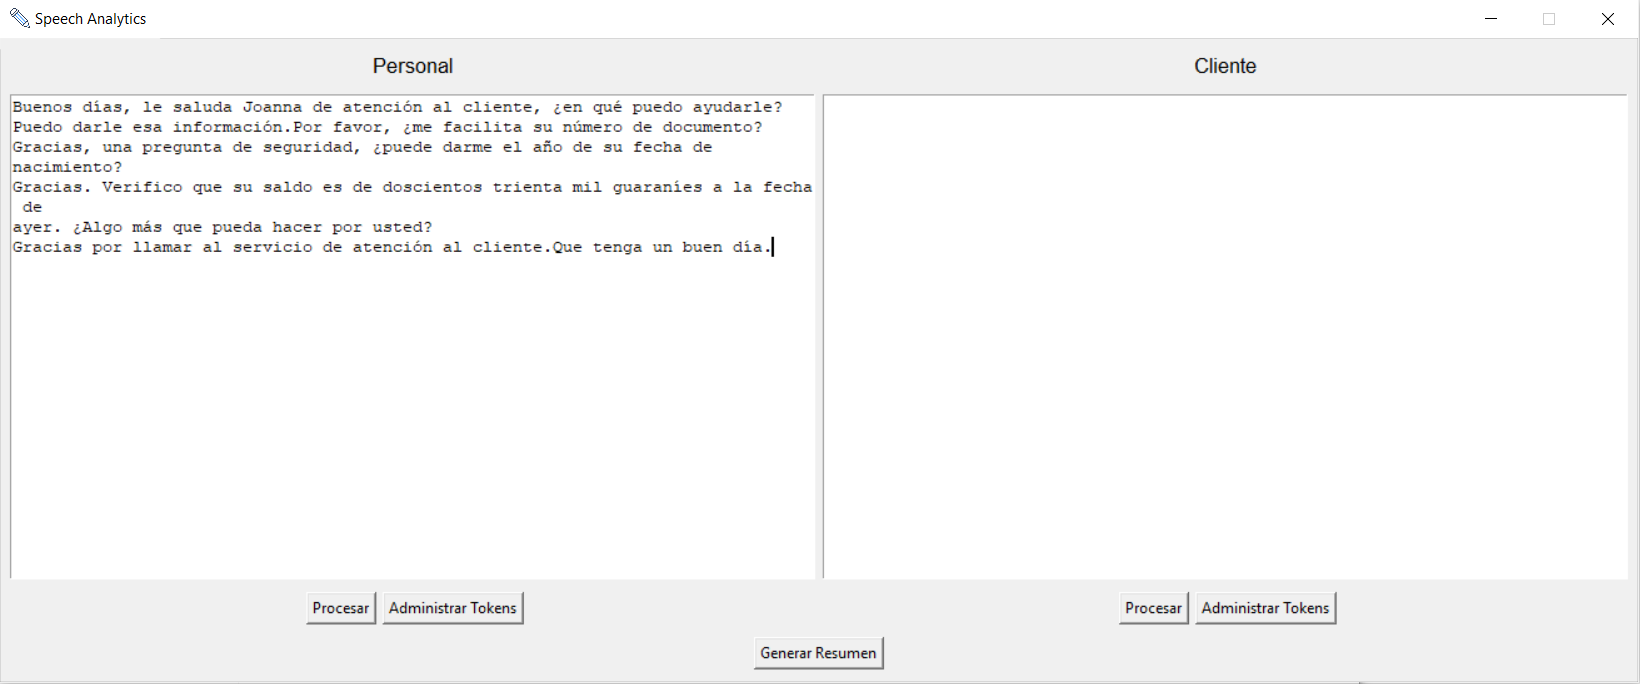
\includegraphics[width=\linewidth]{fig/ATC_paso1.png}
    \caption{Ingreso de datos del personal}
    \label{fig:graf_atc_paso1}
\end{figure}

\subsubsection{Procesamos el texto}
A continuación, se presiona el botón \textbf{Procesar} correspondiente al personal, tal como se muestra en la Figura \ref{fig:graf_atc_paso2}.

\begin{figure}[H]
    \centering
    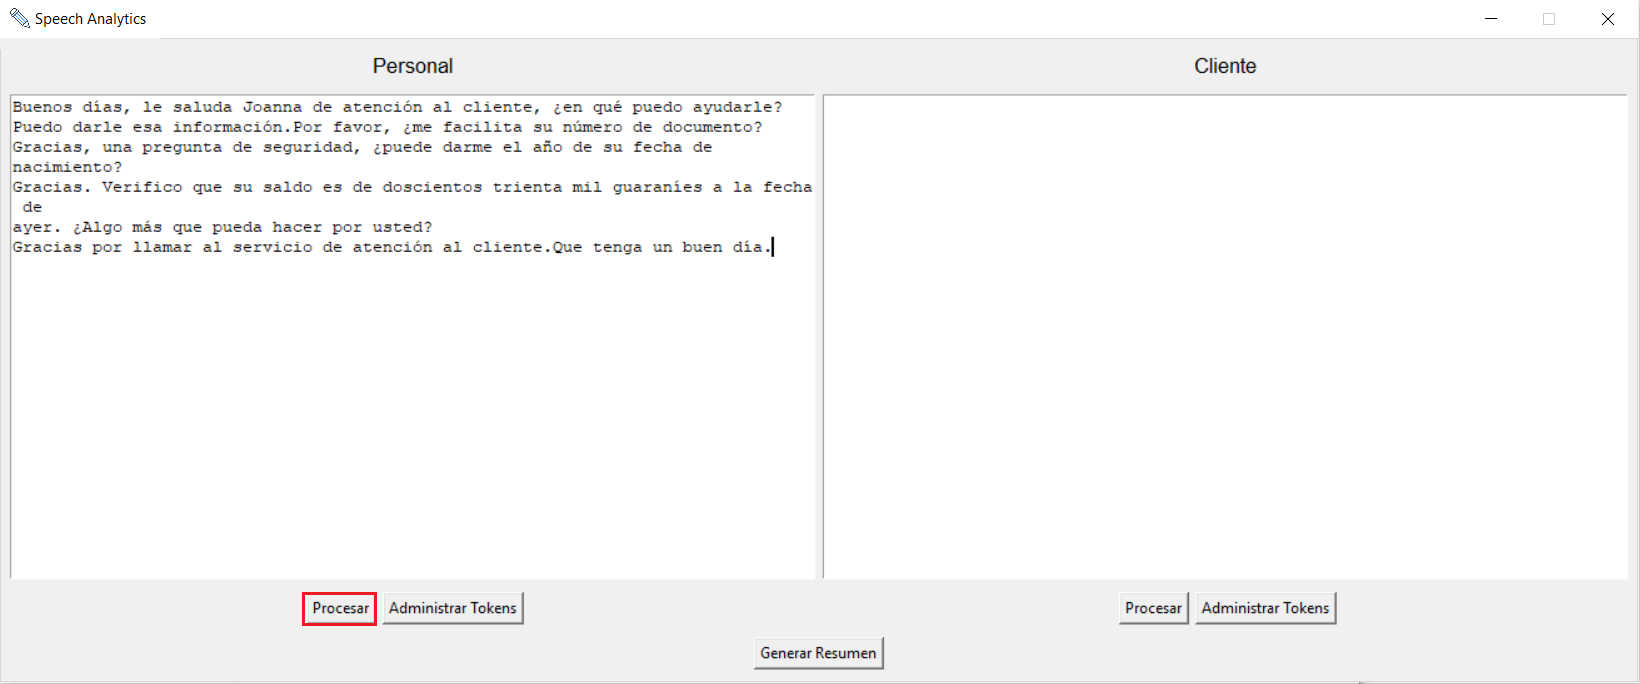
\includegraphics[width=\linewidth]{fig/ATC_paso2.png}
    \caption{Procesamiento del texto ingresado}
    \label{fig:graf_atc_paso2}
\end{figure}

\subsubsection{Categorización de los lexemas}
Al principio, es necesario entrenar el programa, ya que aún no tiene cargada ninguna información. Por lo tanto, debemos indicarle palabra por palabra a qué token pertenecen, tal y como se observa en la Figura \ref{fig:graf_atc_paso3}.

\begin{figure}[H]
    \centering
    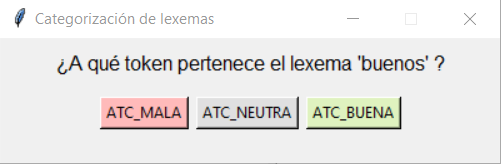
\includegraphics[width=\linewidth]{fig/ATC_paso3.png}
    \caption{Categorización de los lexemas}
    \label{fig:graf_atc_paso3}
\end{figure}

\subsubsection{Resultados preliminares}
Una vez completado el paso anterior, podremos observar los resultados generados para este análisis, los cuales se ajustarán a los criterios establecidos previamente. En la Figura \ref{fig:graf_atc_paso4}, podremos observar esto. Estos resultados nos proporcionan información sobre el desempeño del personal de ATC y nos permiten identificar si es necesario realizar mejoras en su capacitación.

\begin{figure}[H]
    \centering
    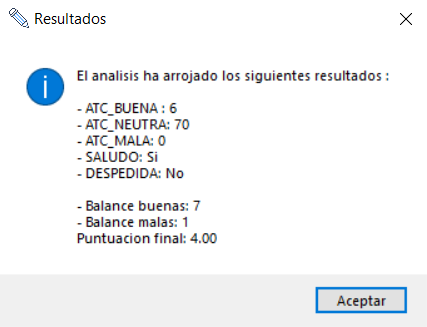
\includegraphics[width=\linewidth]{fig/ATC_paso4.png}
    \caption{Resultados del análisis}
    \label{fig:graf_atc_paso4}
\end{figure}

En la pantalla principal también podremos visualizar los resultados de manera gráfica de la categorización, tal y como se muestra en la Figura \ref{fig:graf_atc_paso5}. En donde el color de resaltado indica el token al que pertenece la palabra.

\begin{figure}[H]
    \centering
    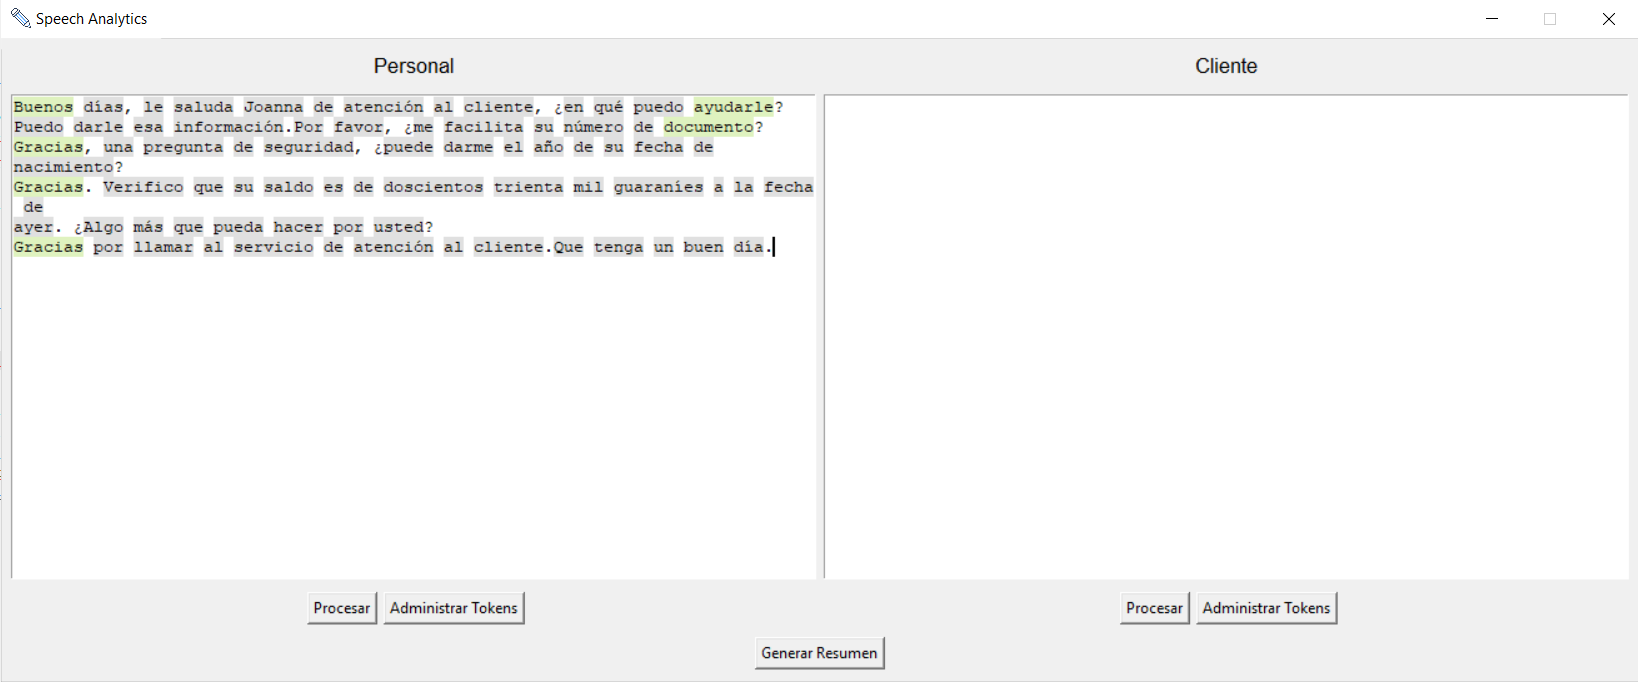
\includegraphics[width=\linewidth]{fig/ATC_paso5.png}
    \caption{Resultado de la categorización}
    \label{fig:graf_atc_paso5}
\end{figure}

\subsubsection{Administración de tokens}
Una vez procesado el texto, también podemos gestionar los tokens de las palabras reconocidas en el texto. Es decir, tenemos la opción de cambiar los tokens ya establecidos para que el tokenizador pueda actualizar su base de datos y aprender conforme vayamos estableciendo los parámetros. Para acceder a esta función, simplemente hacemos clic en el botón \textbf{Administrar Tokens}, como se muestra en la Figura \ref{fig:graf_atc_paso6}.

\begin{figure}[H]
    \centering
    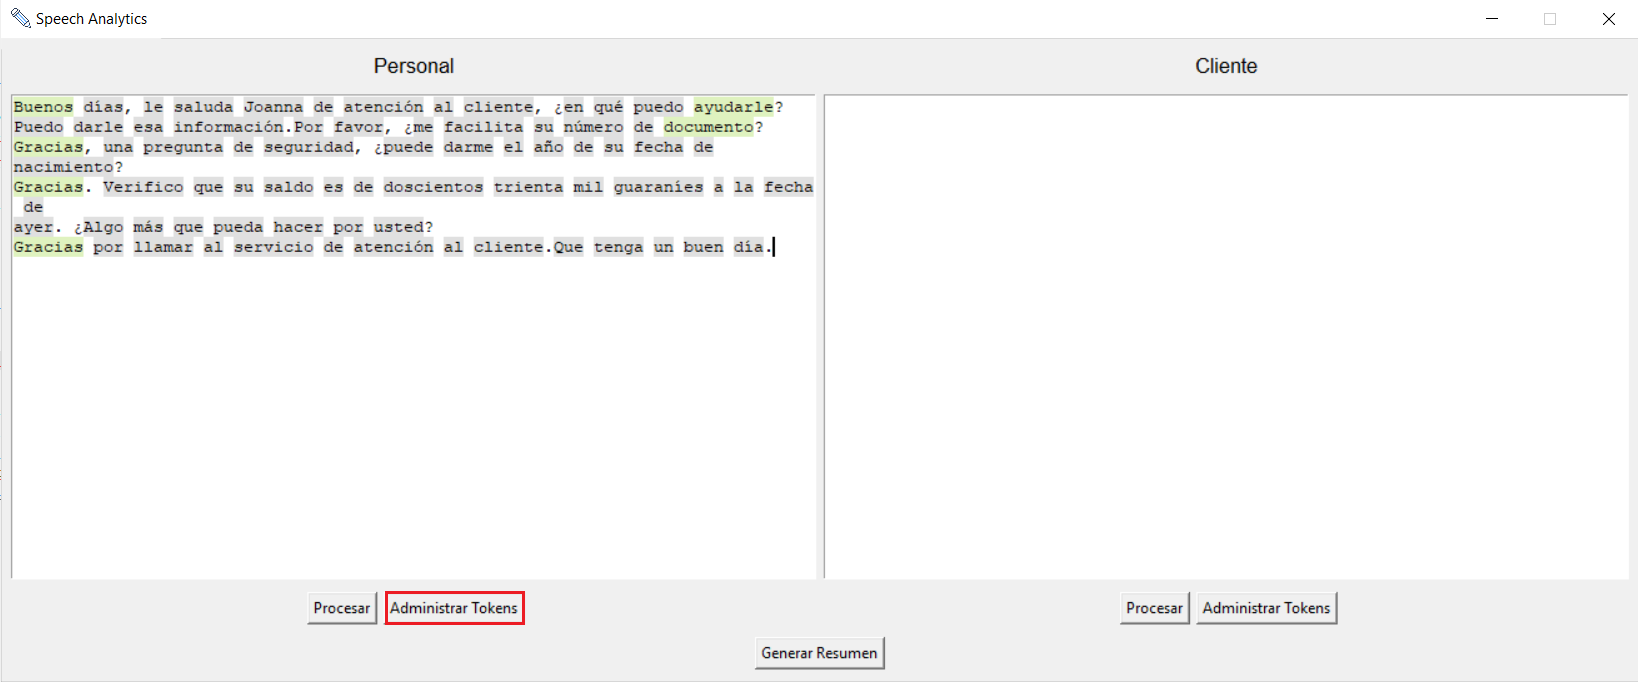
\includegraphics[width=\linewidth]{fig/ATC_paso6.png}
    \caption{Administración de tokens}
    \label{fig:graf_atc_paso6}
\end{figure}

A continuación, se desplegará la ventana de administración de tokens, donde tendremos la capacidad de modificar el token asociado al lexema reconocido, tal y como se puede observar en la Figura \ref{fig:graf_atc_paso7}.

\begin{figure}[H]
    \centering
    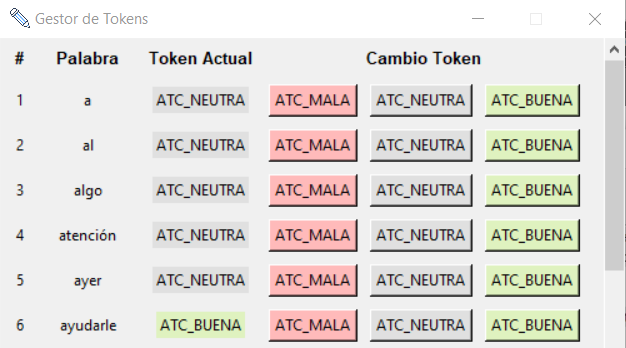
\includegraphics[width=0.5\textwidth]{fig/ATC_paso7.png}
    \caption{Ventana del administrador de tokens}
    \label{fig:graf_atc_paso7}
\end{figure}

\subsection{Procesamiento de la interacción del Cliente}
Todos los pasos descritos anteriormente para la interacción del personal de atención al cliente (ATC) se repiten para el cliente. El resultado final se puede observar en la Figura \ref{fig:graf_cliente_resultados}. Esta información es útil para determinar la calidad del servicio ofrecido.

\begin{figure}[H]
    \centering
    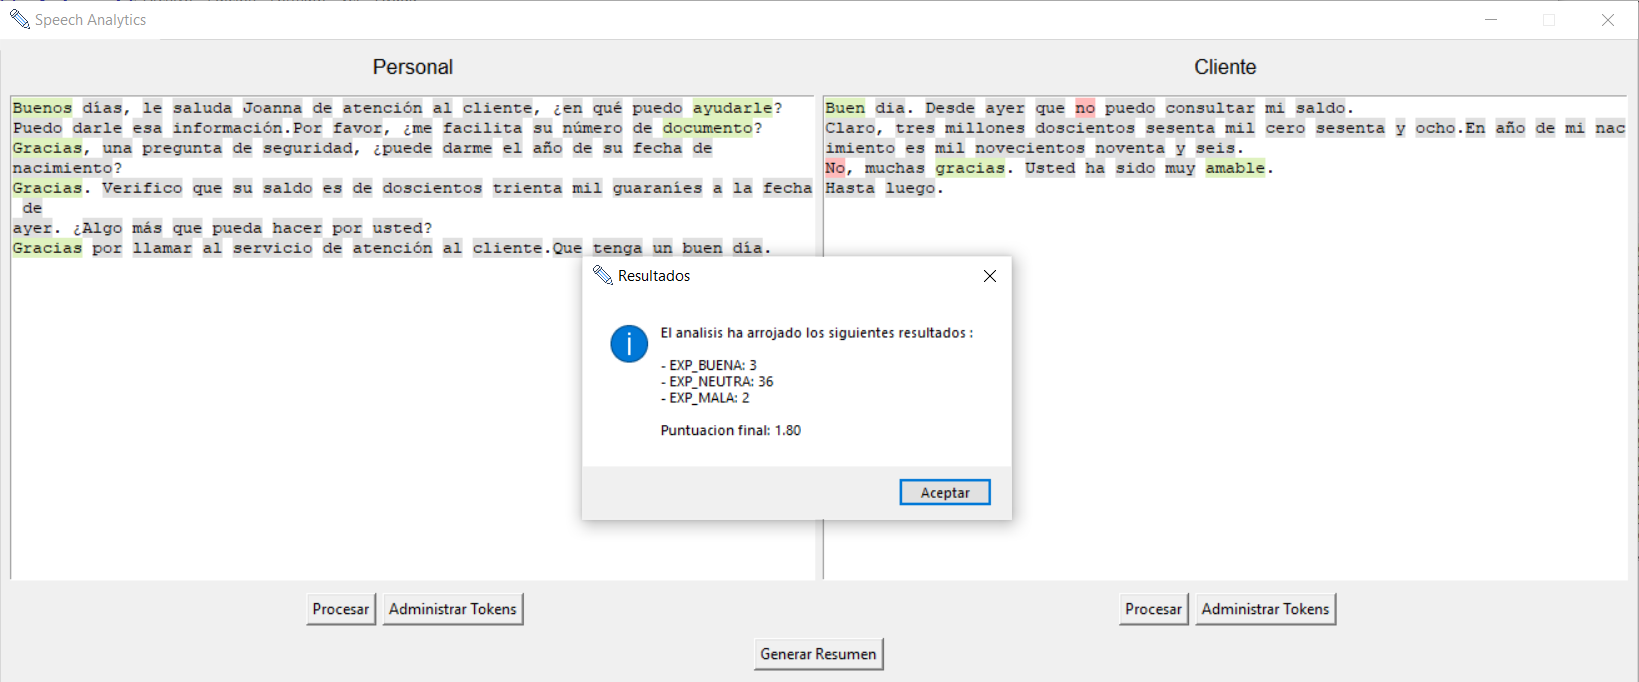
\includegraphics[width=0.5\textwidth]{fig/cliente_resultados.png}
    \caption{Ventana del administrador de tokens}
    \label{fig:graf_cliente_resultados}
\end{figure}

\subsection{Resultado y puntuación general de la interacción}
A continuación, para generar el resumen general de la interacción, debemos presionar el botón \textbf{Generar Resumen}, como se muestra en la Figura \ref{fig:graf_resumen_general}.

\begin{figure}[H]
    \centering
    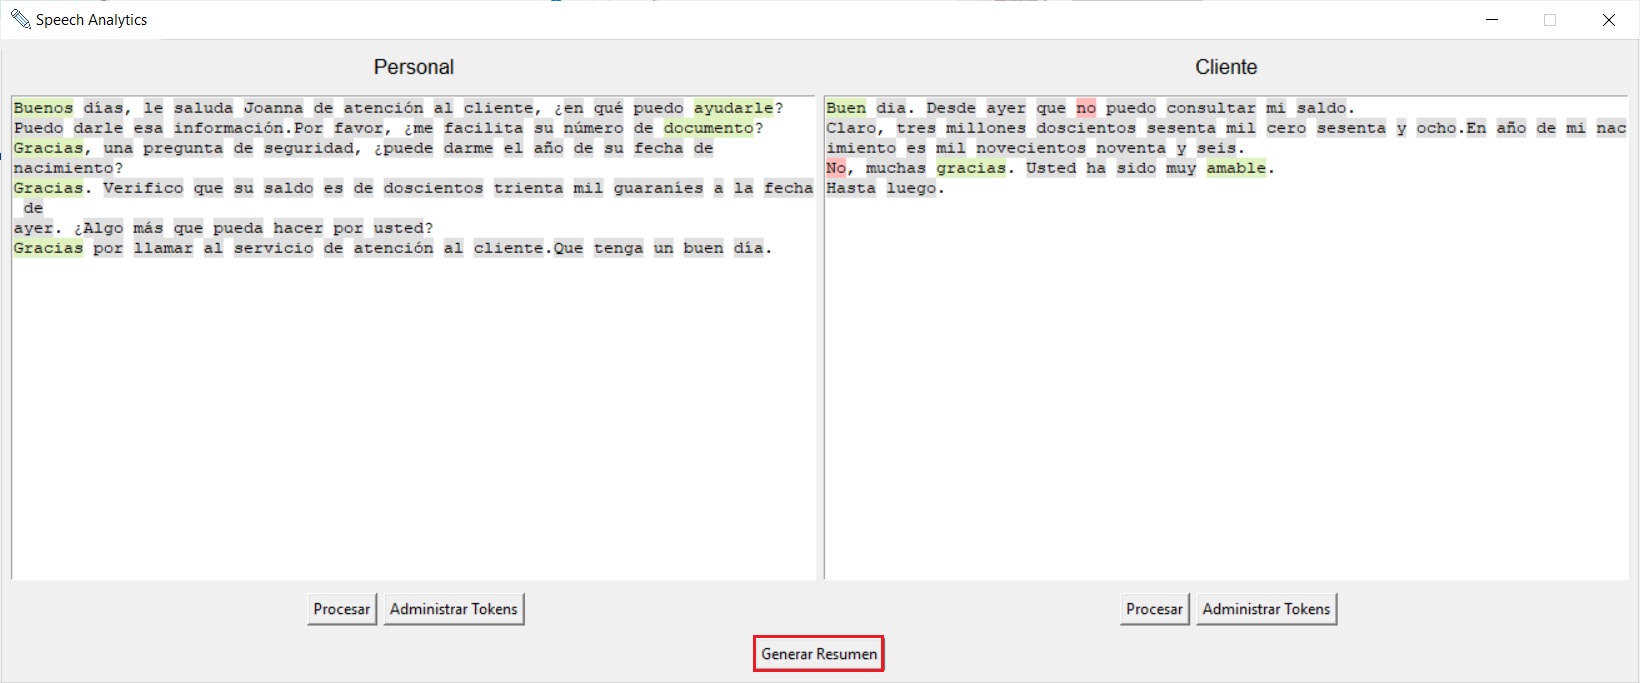
\includegraphics[width=0.5\textwidth]{fig/resumen_general.png}
    \caption{Generación del resumen general}
    \label{fig:graf_resumen_general}
\end{figure}

Esto nos generará un resumen de la interacción de la llamada entre el ATC y el cliente. Esta puntuación es un promedio de ambas interacciones y nos proporciona una noción de la puntuación general de la llamada realizada. El resultado se puede observar en la Figura \ref{fig:graf_resultado_general}.

\begin{figure}[H]
    \centering
    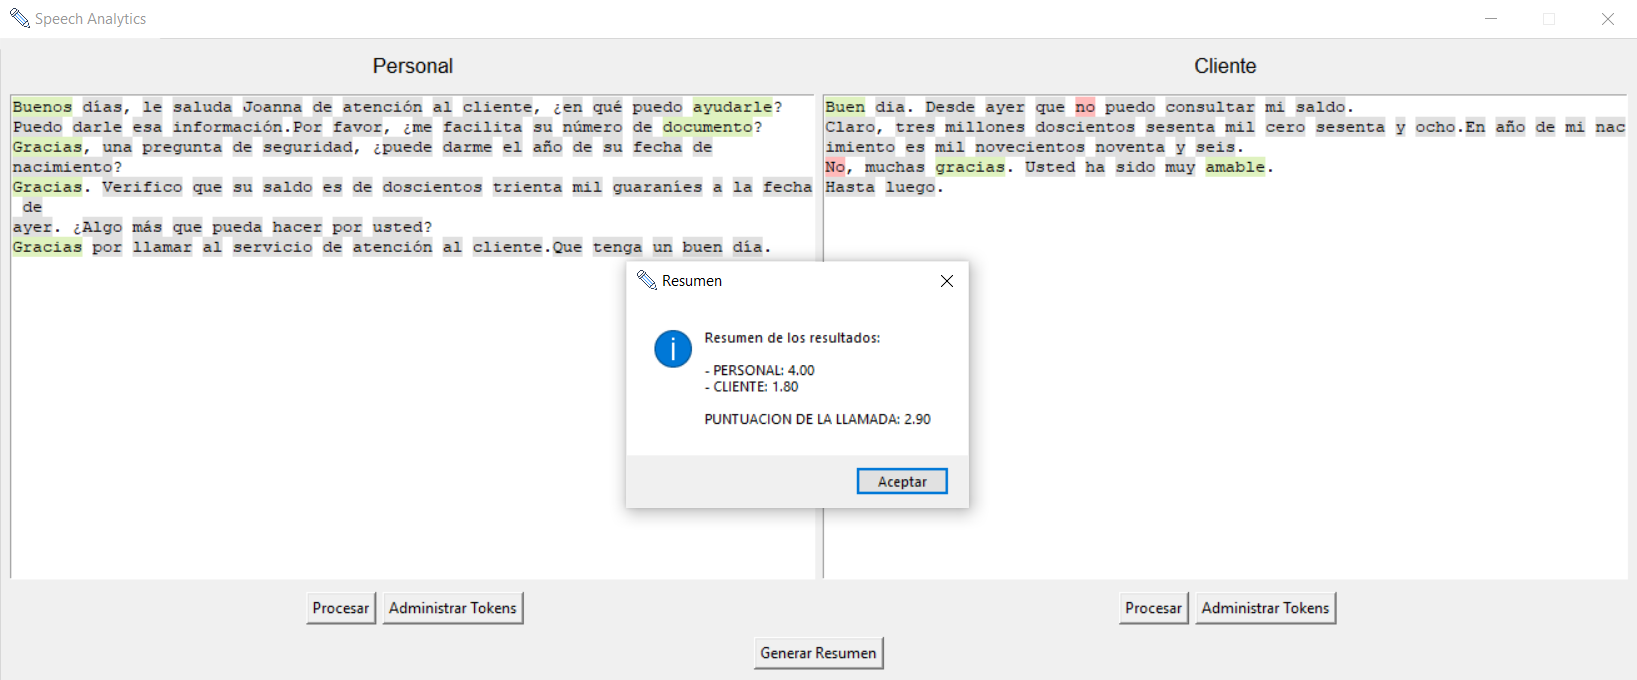
\includegraphics[width=0.5\textwidth]{fig/resultado_general.png}
    \caption{Generación del resumen general}
    \label{fig:graf_resultado_general}
\end{figure}

\printbibliography

\end{document}